
\clearpage{}
% -----------------------------------------------------------------------------
\section{Privacy}
\label{s:Privacy}

\begin{figure}
\begin{center}
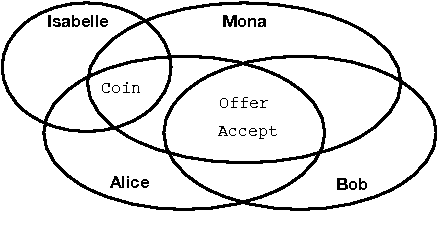
\includegraphics{figure/coin-transfer-visibility.pdf}
\end{center}
\vspace{-2ex}
\caption{Fact Visibility in Coin Transfer Example}
\label{f:CoinTransferVisibility}
\end{figure}

In many practical commercial workflows, it is either not desirable or not legal for all parties to be able to see all data in the system. In the coin transfer example from \S\ref{s:FactsWeights}, suppose that Alice wishes to transfer a coin to Bob, but does not want to reveal the total number of coins she holds. Recall from \S\ref{s:Observation} that a party can see a fact when it is listed in either its \emph{by-authority} set or its \emph{obs-authority} set. We can express this as a simple predicate, where the functions \trm{auth-by} and \trm{auth-obs} retrieve the respective metadata from a fact value.
$$
\trm{sees}~ P~ F = |(\trm{auth-by}~F \cup \trm{auth-obs}~F) \cap \{P\}| \ge 0
$$
Applying this predicate to the initial facts from \S\ref{s:NowWithMetadata} we see that we already have the desired situation. The coin fact and its weight is visible to Alice (the giver), and Mona (the monitor), while the Offer and Accept facts are visible to all three of Alice, Bob and Mona. Figure~\ref{f:CoinTransferVisibility} shows this in diagrammatic form.


\subsection{Transactions and Validation}
Maintaining fact privacy has implications for the underlying implementation. Assume that Alice, Bob and Mona all have their own computers in their own offices that each initially contain the subset of facts that each can see as per Figure~\ref{f:CoinTransferVisibility}. Assume that each party also has a copy of the transfer rule shown in Figure~\ref{f:CoinTransfer}. Now, suppose Alice decides that it is time to perform the transfer. On her own computer she executes the rule while recording the facts that have been consumed and the new facts that have been produced. She then builds a transaction data structure that records this information along with the cryptographic hash of the rule code, which we describe as so:

\begin{small}
\begin{code}
Transaction
{ ident = ... fresh number ...
, rule  = ... hash of code for transfer rule ...
, spent
   = [ Offer  [id = '1234, give = !Alice, recv = !Bob]
        by  {!Bob}              obs {!Mona, !Alice}
        use {'transfer}         num 1

     , Accept [id = '1234, acc = !Bob]
        by  {!Alice}            obs {!Mona, !Bob}
        use {'transfer}         num 1

     , Coin   [issuer = !Isabelle, holder = !Alice]
        by  {!Isabelle, !Alice} obs {!Mona}
        use {'transfer}         num 1 ]
, new
   = [ Coin   [issuer = !Isabelle, holder = !Bob]
        by  {!Isabelle, !Bob}   obs {!Mona}
        use {'transfer}         num 1 ]
\end{code}
\end{small}

This is the complete transaction that describes all inputs and outputs. For now, we will broadcast the entire transaction as to all parties in the network. In the next section we will discuss how to ensure that parties are only able to see the input and output facts that they are observers for.

\subsection{Blinded Transactions}
Alice can send the complete transaction to Mona, which is also entitled to see all the input and output facts, however we cannot also sent it to Isabelle and Bob because they are not entitled to see some of the components.

Instead, we can compute a \emph{restricted view} of the transaction for both Isabelle and Bob, which consists of a blinded hash of the entire transaction, along with a version of the transaction structure where the facts that a particular party are not entitled to see are replaced by blinded hashes of those facts. A \emph{blinded} hash is a regular cryptographic hash which has been combined with a salt value so that it cannot be easilly brute forced.

\TODO{In above transaction the meta-data reveals that it can be formally seen by Isabelle, Bob and Mona, though of course Alice knows about it as she built the transaction}. Distinguish between observer, formal observer, and incidental observer. As Alice is only an incidental observer she should not retain the fact data, as she will not receive information about transactions that spend this fact. Any transactions she might form based on this information may be invalid without her knowing.










